% Options for packages loaded elsewhere
\PassOptionsToPackage{unicode}{hyperref}
\PassOptionsToPackage{hyphens}{url}
%
\documentclass[
]{article}
\usepackage{amsmath,amssymb}
\usepackage{iftex}
\ifPDFTeX
  \usepackage[T1]{fontenc}
  \usepackage[utf8]{inputenc}
  \usepackage{textcomp} % provide euro and other symbols
\else % if luatex or xetex
  \usepackage{unicode-math} % this also loads fontspec
  \defaultfontfeatures{Scale=MatchLowercase}
  \defaultfontfeatures[\rmfamily]{Ligatures=TeX,Scale=1}
\fi
\usepackage{lmodern}
\ifPDFTeX\else
  % xetex/luatex font selection
\fi
% Use upquote if available, for straight quotes in verbatim environments
\IfFileExists{upquote.sty}{\usepackage{upquote}}{}
\IfFileExists{microtype.sty}{% use microtype if available
  \usepackage[]{microtype}
  \UseMicrotypeSet[protrusion]{basicmath} % disable protrusion for tt fonts
}{}
\makeatletter
\@ifundefined{KOMAClassName}{% if non-KOMA class
  \IfFileExists{parskip.sty}{%
    \usepackage{parskip}
  }{% else
    \setlength{\parindent}{0pt}
    \setlength{\parskip}{6pt plus 2pt minus 1pt}}
}{% if KOMA class
  \KOMAoptions{parskip=half}}
\makeatother
\usepackage{xcolor}
\usepackage[margin=1in]{geometry}
\usepackage{color}
\usepackage{fancyvrb}
\newcommand{\VerbBar}{|}
\newcommand{\VERB}{\Verb[commandchars=\\\{\}]}
\DefineVerbatimEnvironment{Highlighting}{Verbatim}{commandchars=\\\{\}}
% Add ',fontsize=\small' for more characters per line
\usepackage{framed}
\definecolor{shadecolor}{RGB}{248,248,248}
\newenvironment{Shaded}{\begin{snugshade}}{\end{snugshade}}
\newcommand{\AlertTok}[1]{\textcolor[rgb]{0.94,0.16,0.16}{#1}}
\newcommand{\AnnotationTok}[1]{\textcolor[rgb]{0.56,0.35,0.01}{\textbf{\textit{#1}}}}
\newcommand{\AttributeTok}[1]{\textcolor[rgb]{0.13,0.29,0.53}{#1}}
\newcommand{\BaseNTok}[1]{\textcolor[rgb]{0.00,0.00,0.81}{#1}}
\newcommand{\BuiltInTok}[1]{#1}
\newcommand{\CharTok}[1]{\textcolor[rgb]{0.31,0.60,0.02}{#1}}
\newcommand{\CommentTok}[1]{\textcolor[rgb]{0.56,0.35,0.01}{\textit{#1}}}
\newcommand{\CommentVarTok}[1]{\textcolor[rgb]{0.56,0.35,0.01}{\textbf{\textit{#1}}}}
\newcommand{\ConstantTok}[1]{\textcolor[rgb]{0.56,0.35,0.01}{#1}}
\newcommand{\ControlFlowTok}[1]{\textcolor[rgb]{0.13,0.29,0.53}{\textbf{#1}}}
\newcommand{\DataTypeTok}[1]{\textcolor[rgb]{0.13,0.29,0.53}{#1}}
\newcommand{\DecValTok}[1]{\textcolor[rgb]{0.00,0.00,0.81}{#1}}
\newcommand{\DocumentationTok}[1]{\textcolor[rgb]{0.56,0.35,0.01}{\textbf{\textit{#1}}}}
\newcommand{\ErrorTok}[1]{\textcolor[rgb]{0.64,0.00,0.00}{\textbf{#1}}}
\newcommand{\ExtensionTok}[1]{#1}
\newcommand{\FloatTok}[1]{\textcolor[rgb]{0.00,0.00,0.81}{#1}}
\newcommand{\FunctionTok}[1]{\textcolor[rgb]{0.13,0.29,0.53}{\textbf{#1}}}
\newcommand{\ImportTok}[1]{#1}
\newcommand{\InformationTok}[1]{\textcolor[rgb]{0.56,0.35,0.01}{\textbf{\textit{#1}}}}
\newcommand{\KeywordTok}[1]{\textcolor[rgb]{0.13,0.29,0.53}{\textbf{#1}}}
\newcommand{\NormalTok}[1]{#1}
\newcommand{\OperatorTok}[1]{\textcolor[rgb]{0.81,0.36,0.00}{\textbf{#1}}}
\newcommand{\OtherTok}[1]{\textcolor[rgb]{0.56,0.35,0.01}{#1}}
\newcommand{\PreprocessorTok}[1]{\textcolor[rgb]{0.56,0.35,0.01}{\textit{#1}}}
\newcommand{\RegionMarkerTok}[1]{#1}
\newcommand{\SpecialCharTok}[1]{\textcolor[rgb]{0.81,0.36,0.00}{\textbf{#1}}}
\newcommand{\SpecialStringTok}[1]{\textcolor[rgb]{0.31,0.60,0.02}{#1}}
\newcommand{\StringTok}[1]{\textcolor[rgb]{0.31,0.60,0.02}{#1}}
\newcommand{\VariableTok}[1]{\textcolor[rgb]{0.00,0.00,0.00}{#1}}
\newcommand{\VerbatimStringTok}[1]{\textcolor[rgb]{0.31,0.60,0.02}{#1}}
\newcommand{\WarningTok}[1]{\textcolor[rgb]{0.56,0.35,0.01}{\textbf{\textit{#1}}}}
\usepackage{graphicx}
\makeatletter
\def\maxwidth{\ifdim\Gin@nat@width>\linewidth\linewidth\else\Gin@nat@width\fi}
\def\maxheight{\ifdim\Gin@nat@height>\textheight\textheight\else\Gin@nat@height\fi}
\makeatother
% Scale images if necessary, so that they will not overflow the page
% margins by default, and it is still possible to overwrite the defaults
% using explicit options in \includegraphics[width, height, ...]{}
\setkeys{Gin}{width=\maxwidth,height=\maxheight,keepaspectratio}
% Set default figure placement to htbp
\makeatletter
\def\fps@figure{htbp}
\makeatother
\setlength{\emergencystretch}{3em} % prevent overfull lines
\providecommand{\tightlist}{%
  \setlength{\itemsep}{0pt}\setlength{\parskip}{0pt}}
\setcounter{secnumdepth}{-\maxdimen} % remove section numbering
\ifLuaTeX
  \usepackage{selnolig}  % disable illegal ligatures
\fi
\IfFileExists{bookmark.sty}{\usepackage{bookmark}}{\usepackage{hyperref}}
\IfFileExists{xurl.sty}{\usepackage{xurl}}{} % add URL line breaks if available
\urlstyle{same}
\hypersetup{
  pdftitle={Projet d'étude : Analyse de données \& Éléments de modélisation statistique},
  hidelinks,
  pdfcreator={LaTeX via pandoc}}

\title{Projet d'étude : Analyse de données \& Éléments de modélisation
statistique}
\author{}
\date{\vspace{-2.5em}2023-09-29}

\begin{document}
\maketitle

\begin{verbatim}
## corrplot 0.92 loaded
\end{verbatim}

\hypertarget{statistiques-descriptives}{%
\section{Statistiques descriptives}\label{statistiques-descriptives}}

Le jeu de données comprend \(984\) mesures des émissions de polluants
atmosphériques tous secteurs d'activités confondues des EPCI
(Etablissements Publics de Coopération Intercommunale) de la région
Occitanie de 2014 à 2019.

Chaque mesure est décrite par les variables qualitatives suivantes : +
\emph{lib\_epci} : son nom + \emph{code\_epci} : son code
d'identification + \emph{nomdepart} : son (ses) département(s)
d'appartenance + \emph{TypeEPCI} : CC (communauté de commune), CA
(communauté d'agglomération), Métrople et CU (communauté urbaine) +
\emph{annee\_inv} : l'année de mesure

Et par les variables quantitatives suivantes : + \emph{nox\_kg} : oxyde
d'azote en kg + \emph{so2\_kg} : oxyde de soufre en kg + \emph{pm10\_kg}
: particules en suspension dans l'air de diamètre inférieur à 10 µm +
\emph{pm25\_kg} : particules en suspension dans l'air de diamètre
inférieur à 2.5 µm + \emph{co\_kg} : monoxyde de carbone +
\emph{c6h6\_kg} : benzène + \emph{nh3\_kg} : ammoniac +
\emph{ges\_teqco2} : gaz à effet de serre + \emph{ch4\_t} : méthane +
\emph{co2\_t} : dioxyde de carbone + \emph{n2o\_t} : protoxyde d'azote +
\emph{latit} : sa latitude + \emph{longit} : sa longitude

Dans la suite de ce rapport, nous utilisons la notation \(\Delta\) pour
faire référence à des plots qui sont disponibles dans le Rmd mais que
nous avons décidé de ne pas inclure dans le rapport.

\begin{verbatim}
##   code_epci                            lib_epci annee_inv     nox_kg    so2_kg
## 1 200006930                   CC du Haut Allier      2019   65633.66  3866.599
## 2 200017341               CC Lodévois et Larzac      2019  310288.20  8083.028
## 3 200022986          CC du Grand Pic Saint-Loup      2019  337655.55  9373.106
## 4 200023620       CC de la Gascogne Toulousaine      2019  298100.30  4091.852
## 5 200023737                  CA du Grand Cahors      2019  447186.53 13650.148
## 6 200027183 CU Perpignan Méditerranée Métropole      2019 2110865.51 57993.192
##     pm10_kg   pm25_kg     co_kg   c6h6_kg    nh3_kg ges_teqco2   ch4_t
## 1  15728.87  10975.55  173194.3  2319.199 133686.18   43995.12 617.104
## 2  50929.20  38591.71  593036.6  8349.081 114533.40  127777.47 436.445
## 3 143623.67  82143.61 1275976.8 18806.497  71177.45  161136.84 251.623
## 4 126735.60  63331.88  780230.6 12250.430 244266.82  116802.18 275.749
## 5 143525.58 111854.31 1386798.2 21346.289 130426.82  216301.79 447.677
## 6 506888.15 353513.88 5270166.1 78510.229 111010.72 1057760.61 398.561
##       co2_t  n2o_t TypeEPCI           nomdepart Ardèche Ariège Aude Aveyron
## 1  17831.59 17.114       CC              Lozère       0      0    0       0
## 2  93016.70 19.755       CC             Hérault       0      0    0       0
## 3 125004.72 17.606       CC             Hérault       0      0    0       0
## 4  79458.03 50.976       CC  Gers,Haute-Garonne       0      0    0       0
## 5 161747.97 24.640       CA                 Lot       0      0    0       0
## 6 806673.97 59.760       CU Pyrénées-Orientales       0      0    0       0
##   Gard Haute.Garonne Gers Hérault Landes Lot Lot.et.Garonne Lozère
## 1    0             0    0       0      0   0              0      1
## 2    0             0    0       1      0   0              0      0
## 3    0             0    0       1      0   0              0      0
## 4    0             1    1       0      0   0              0      0
## 5    0             0    0       0      0   1              0      0
## 6    0             0    0       0      0   0              0      0
##   Pyrénées.Atlantiques Hautes.Pyrénées Pyrénées.Orientales Tarn Tarn.et.Garonne
## 1                    0               0                   0    0               0
## 2                    0               0                   0    0               0
## 3                    0               0                   0    0               0
## 4                    0               0                   0    0               0
## 5                    0               0                   0    0               0
## 6                    0               0                   1    0               0
##   Vaucluse    latit   longit
## 1        0 44.73240 3.769267
## 2        0 43.79291 3.372977
## 3        0 43.77692 3.794306
## 4        0 43.59144 1.066752
## 5        0 44.48480 1.447761
## 6        0 42.75200 2.851604
\end{verbatim}

\hypertarget{analyse-unidimentionnelle}{%
\subsection{Analyse unidimentionnelle}\label{analyse-unidimentionnelle}}

\hypertarget{analyse-des-variables-quantitatives}{%
\subsubsection{Analyse des variables
quantitatives}\label{analyse-des-variables-quantitatives}}

Nous observons avec ce boxplot que nos variables n'ont pas les mêmes
échelles de valeur (MODIF : ordres de grandeur), cela va biaiser nos
analyses de variances. Nous appliquons donc une transformation
logarithmique aux valeurs quantitatives.

\begin{verbatim}
## No id variables; using all as measure variables
\end{verbatim}

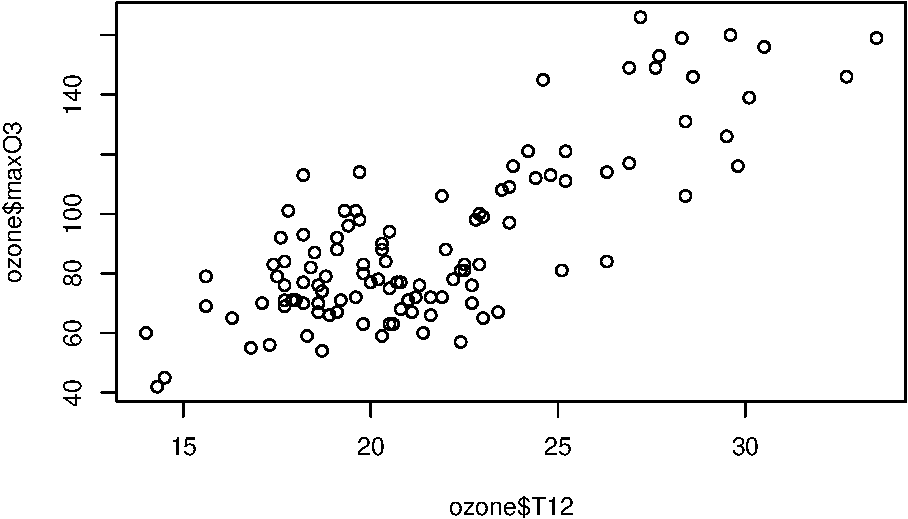
\includegraphics{rool-nguyen-gourio-moshfeghi-Rapport_files/figure-latex/unnamed-chunk-6-1.pdf}

Nous stockons le dataset avec les variables quantitatives transformées
dans la variable \(Datalog\).

Nous remarquons que la transformation logarithme suffit à mieux
visualiser nos données. Nous utiliserons ce jeu de données par la suite.

\begin{verbatim}
## No id variables; using all as measure variables
\end{verbatim}

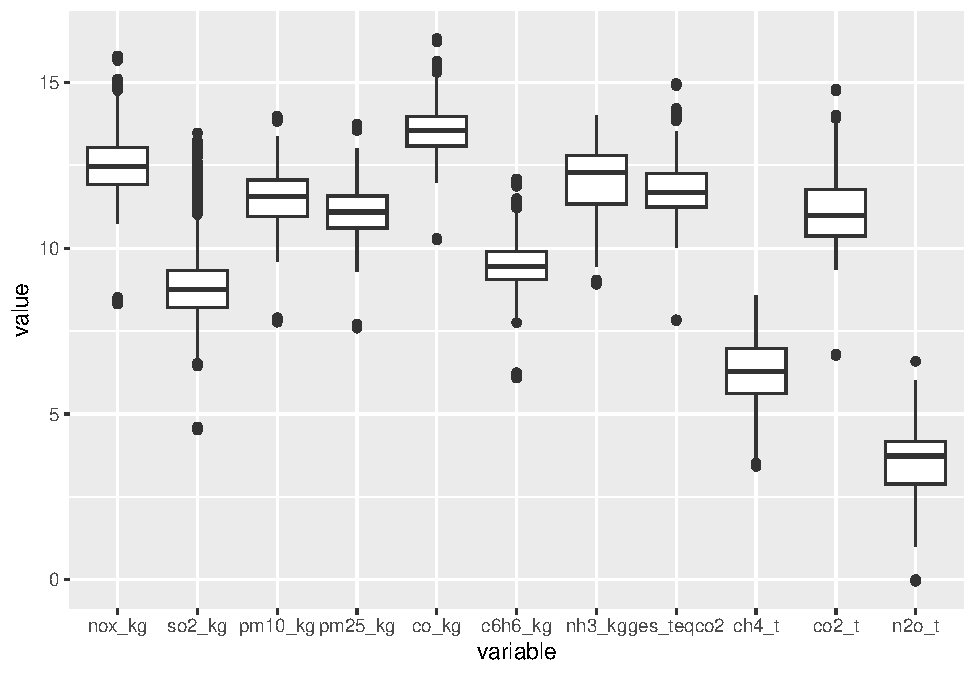
\includegraphics{rool-nguyen-gourio-moshfeghi-Rapport_files/figure-latex/unnamed-chunk-8-1.pdf}

Nous affichons maintenant la fonction de répartition de la concentration
d'oxyde d'azote.

\((\Delta)\) D'autres graphes similaires sont disponibles dans le Rmd.

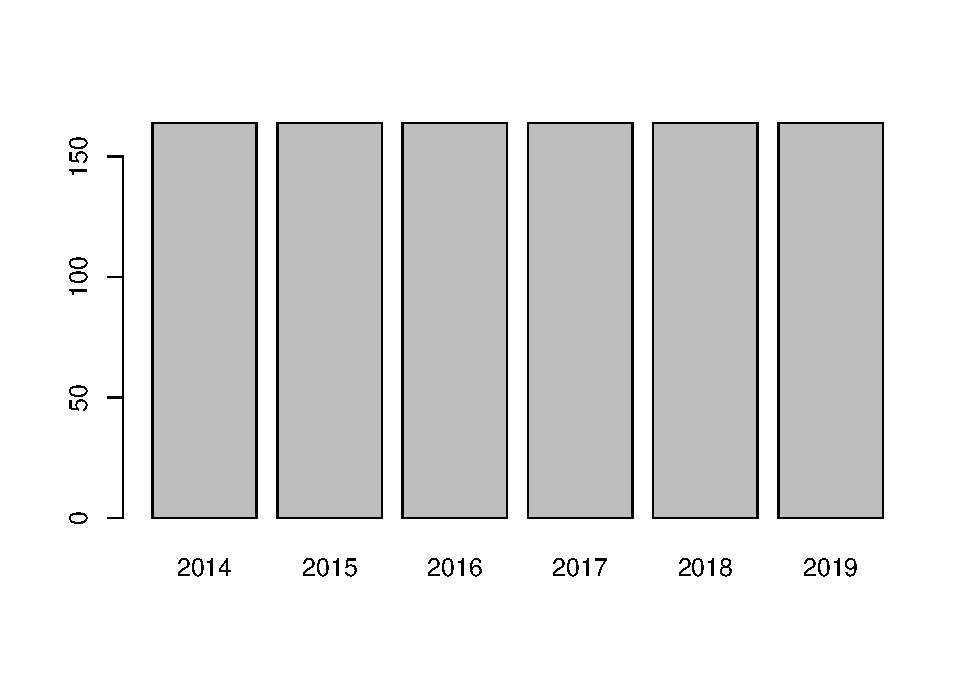
\includegraphics{rool-nguyen-gourio-moshfeghi-Rapport_files/figure-latex/unnamed-chunk-10-1.pdf}

Les données sont uniformément réparties. Cela confirme que nous n'avons
pas besoin d'appliquer d'autres transformations aux variables
quantitatives.

\hypertarget{analyse-des-variables-qualitatives}{%
\subsubsection{Analyse des variables
qualitatives}\label{analyse-des-variables-qualitatives}}

Nous nous intéressons maintenant aux variables qualitatives :
\(TypeEPCI\) \& \(annee_inv\). \((\Delta)\) Nous remarquons que nous
avons le même nombre de prises de mesure pour chaque année, donc aucunes
données ne semblent manquer.

Nous affichons la répartition des mesures en fonction de \(TypeEPCI\).
Nous remarquons que les catégories CA, CU et Metropole ne comprennent
pas beaucoup de valeurs par rapport au type CC. Nous choissisons donc de
combiner les trois catégories pour avoir un nombre suffisant de valeurs
pour chacun de nos différents niveaux.

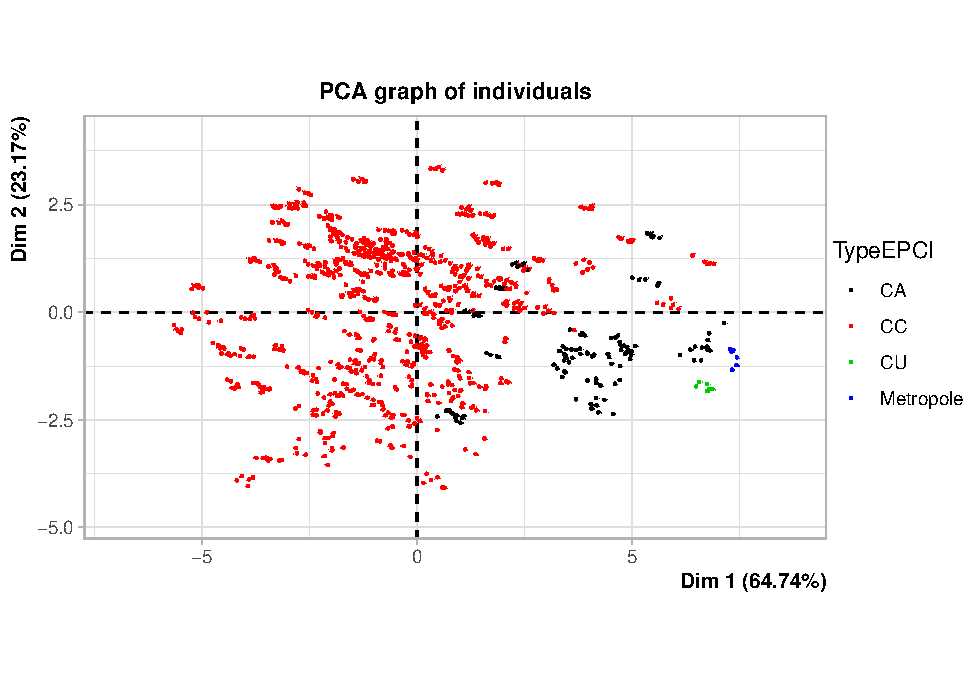
\includegraphics{rool-nguyen-gourio-moshfeghi-Rapport_files/figure-latex/unnamed-chunk-17-1.pdf}

\includegraphics{rool-nguyen-gourio-moshfeghi-Rapport_files/figure-latex/unnamed-chunk-18-1.pdf}

\hypertarget{analyse-bidementionnelle}{%
\subsection{Analyse bidementionnelle}\label{analyse-bidementionnelle}}

En affichant le corrplot, nous observons que tout les polluants sont
corrélés positivement les uns aux autres sauf nh3\_kg, ch4\_t et n2o\_t.
En effet, ces derniers semblents être corrélés seulement qu'entre eux.

\begin{Shaded}
\begin{Highlighting}[]
\FunctionTok{corrplot}\NormalTok{(}\FunctionTok{cor}\NormalTok{(Datalog\_[}\DecValTok{4}\SpecialCharTok{:}\DecValTok{14}\NormalTok{]), }\AttributeTok{method=}\StringTok{"ellipse"}\NormalTok{)}
\end{Highlighting}
\end{Shaded}

\includegraphics{rool-nguyen-gourio-moshfeghi-Rapport_files/figure-latex/unnamed-chunk-19-1.pdf}

\begin{Shaded}
\begin{Highlighting}[]
\FunctionTok{boxplot}\NormalTok{(Datalog}\SpecialCharTok{$}\NormalTok{pm10\_kg}\SpecialCharTok{\textasciitilde{}}\NormalTok{Datalog}\SpecialCharTok{$}\NormalTok{TypeEPCI)}
\end{Highlighting}
\end{Shaded}

\includegraphics{rool-nguyen-gourio-moshfeghi-Rapport_files/figure-latex/unnamed-chunk-20-1.pdf}

\hypertarget{acp}{%
\section{ACP}\label{acp}}

\begin{Shaded}
\begin{Highlighting}[]
\FunctionTok{library}\NormalTok{(mclust)}
\end{Highlighting}
\end{Shaded}

\begin{verbatim}
## Package 'mclust' version 6.0.1
## Type 'citation("mclust")' for citing this R package in publications.
\end{verbatim}

\begin{Shaded}
\begin{Highlighting}[]
\FunctionTok{library}\NormalTok{(cluster)}
\FunctionTok{library}\NormalTok{(factoextra)}
\end{Highlighting}
\end{Shaded}

\begin{verbatim}
## Welcome! Want to learn more? See two factoextra-related books at https://goo.gl/ve3WBa
\end{verbatim}

\begin{Shaded}
\begin{Highlighting}[]
\FunctionTok{library}\NormalTok{(FactoMineR)}
\FunctionTok{library}\NormalTok{(ppclust)}
\FunctionTok{library}\NormalTok{(reticulate)}
\FunctionTok{library}\NormalTok{(ggplot2)}
\FunctionTok{library}\NormalTok{(reshape)}
\end{Highlighting}
\end{Shaded}

\begin{verbatim}
## 
## Attachement du package : 'reshape'
\end{verbatim}

\begin{verbatim}
## Les objets suivants sont masqués depuis 'package:reshape2':
## 
##     colsplit, melt, recast
\end{verbatim}

\begin{Shaded}
\begin{Highlighting}[]
\FunctionTok{library}\NormalTok{(corrplot)}
\FunctionTok{library}\NormalTok{(gridExtra)}
\FunctionTok{library}\NormalTok{(circlize)}
\end{Highlighting}
\end{Shaded}

\begin{verbatim}
## ========================================
## circlize version 0.4.15
## CRAN page: https://cran.r-project.org/package=circlize
## Github page: https://github.com/jokergoo/circlize
## Documentation: https://jokergoo.github.io/circlize_book/book/
## 
## If you use it in published research, please cite:
## Gu, Z. circlize implements and enhances circular visualization
##   in R. Bioinformatics 2014.
## 
## This message can be suppressed by:
##   suppressPackageStartupMessages(library(circlize))
## ========================================
\end{verbatim}

\begin{Shaded}
\begin{Highlighting}[]
\FunctionTok{library}\NormalTok{(viridis)}
\end{Highlighting}
\end{Shaded}

\begin{verbatim}
## Le chargement a nécessité le package : viridisLite
\end{verbatim}

\begin{Shaded}
\begin{Highlighting}[]
\FunctionTok{library}\NormalTok{(reshape2)}
\FunctionTok{library}\NormalTok{(klaR)}
\end{Highlighting}
\end{Shaded}

\begin{verbatim}
## Le chargement a nécessité le package : MASS
\end{verbatim}

Nous réalisons une ACP pour visualiser nos données dans un espace de
dimension inférieure.

Nous remarquons avec les graphes ci-dessous que les deux premières
dimensions constituent 90\% de la variance. Nous allons poursuivre les
analyses par ces deux dimensions.

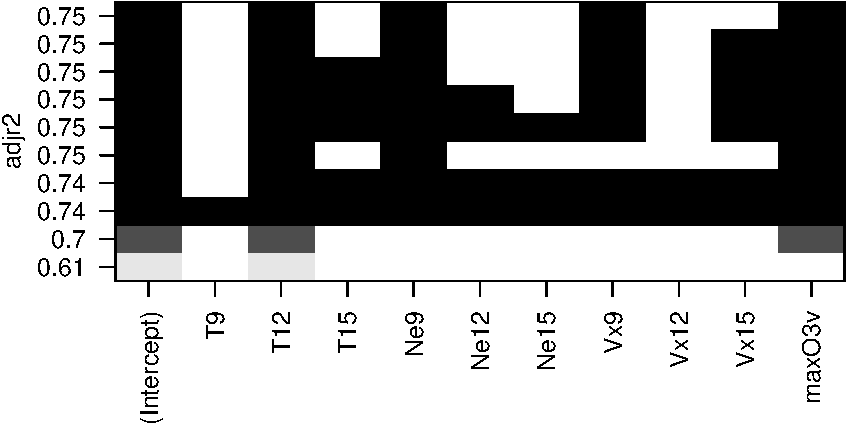
\includegraphics{rool-nguyen-gourio-moshfeghi-Rapport_files/figure-latex/unnamed-chunk-23-1.pdf}
\includegraphics{rool-nguyen-gourio-moshfeghi-Rapport_files/figure-latex/unnamed-chunk-23-2.pdf}

Nous affichons le cercle des corrélations. La première dimension est
consituée de la majorité des polluants sauf ch4\_t, nh3\_kg et n2o\_t
qui constituent la deuxième dimension.

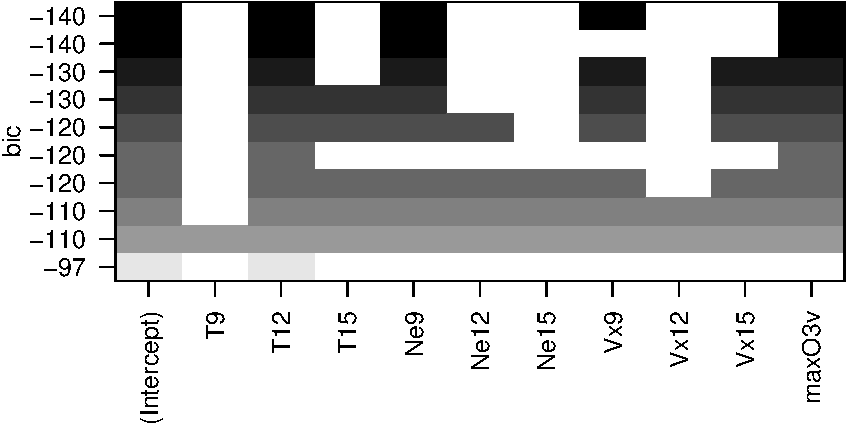
\includegraphics{rool-nguyen-gourio-moshfeghi-Rapport_files/figure-latex/unnamed-chunk-24-1.pdf}

Nous affichons également le graphe des individus colorés en fonction du
Type EPCI. Nous remarquons que les types CA/CU/Metropole ont tendance à
avoir en plus grandes quantité les polluants de la première dimension.
Nous remarquons aussi deux groupements extrêmes. Un groupement très peu
pollué et un autre plus pollué. Après identification, il s'agit de
Toulouse Métropole et de CC Pays de Nay. Nous décidons d'enlever ces
deux groupements car ils ne représentent pas la tendance général ; ce
sont des outliers qui créeront une grande disparité.

\includegraphics{rool-nguyen-gourio-moshfeghi-Rapport_files/figure-latex/unnamed-chunk-25-1.pdf}

\((\Delta)\) Nous affichons aussi cette représentation sans le
groupement des \(TypeEPCI\). Cela confirme que nous avons un classement
de la pollution en fonction du Type EPCI. Si on va du plus au moins
pollué, on a : Metropole, CU, CA puis CC.

\(\Delta\) Nous réaffichons les mêmes graphes sans les deux outliers.

\hypertarget{clustering-pas-ruxe9diguxe9}{%
\section{Clustering (pas rédigé)}\label{clustering-pas-ruxe9diguxe9}}

\begin{Shaded}
\begin{Highlighting}[]
\NormalTok{reskmeans}\OtherTok{\textless{}{-}}\FunctionTok{kmeans}\NormalTok{((Data\_final[,}\DecValTok{4}\SpecialCharTok{:}\DecValTok{14}\NormalTok{]),}\AttributeTok{centers=}\DecValTok{5}\NormalTok{)}
\FunctionTok{table}\NormalTok{(reskmeans}\SpecialCharTok{$}\NormalTok{cluster)}
\end{Highlighting}
\end{Shaded}

\begin{verbatim}
## 
##   1   2   3   4   5 
## 170 296 188 197 121
\end{verbatim}

\begin{Shaded}
\begin{Highlighting}[]
\FunctionTok{fviz\_cluster}\NormalTok{(reskmeans,}\AttributeTok{data=}\NormalTok{Data\_final[,}\DecValTok{4}\SpecialCharTok{:}\DecValTok{14}\NormalTok{],}\AttributeTok{ellipse.type=}\StringTok{"norm"}\NormalTok{,}\AttributeTok{labelsize=}\DecValTok{8}\NormalTok{,}\AttributeTok{geom=}\FunctionTok{c}\NormalTok{(}\StringTok{"point"}\NormalTok{), }\AttributeTok{axes =} \FunctionTok{c}\NormalTok{(}\DecValTok{1}\NormalTok{,}\DecValTok{2}\NormalTok{))}\SpecialCharTok{+}\FunctionTok{ggtitle}\NormalTok{(}\StringTok{""}\NormalTok{)}
\end{Highlighting}
\end{Shaded}

\includegraphics{rool-nguyen-gourio-moshfeghi-Rapport_files/figure-latex/unnamed-chunk-29-1.pdf}

\begin{Shaded}
\begin{Highlighting}[]
\NormalTok{reskmeans}\OtherTok{\textless{}{-}}\FunctionTok{kmeans}\NormalTok{((Datalog[,}\DecValTok{4}\SpecialCharTok{:}\DecValTok{14}\NormalTok{]),}\AttributeTok{centers=}\DecValTok{7}\NormalTok{)}
\FunctionTok{table}\NormalTok{(reskmeans}\SpecialCharTok{$}\NormalTok{cluster)}
\end{Highlighting}
\end{Shaded}

\begin{verbatim}
## 
##   1   2   3   4   5   6   7 
## 180 148 133 212   6 178 127
\end{verbatim}

\begin{Shaded}
\begin{Highlighting}[]
\FunctionTok{fviz\_cluster}\NormalTok{(reskmeans,}\AttributeTok{data=}\NormalTok{Datalog[,}\DecValTok{4}\SpecialCharTok{:}\DecValTok{14}\NormalTok{],}\AttributeTok{ellipse.type=}\StringTok{"norm"}\NormalTok{,}\AttributeTok{labelsize=}\DecValTok{8}\NormalTok{,}\AttributeTok{geom=}\FunctionTok{c}\NormalTok{(}\StringTok{"point"}\NormalTok{), }\AttributeTok{axes =} \FunctionTok{c}\NormalTok{(}\DecValTok{1}\NormalTok{,}\DecValTok{2}\NormalTok{))}\SpecialCharTok{+}\FunctionTok{ggtitle}\NormalTok{(}\StringTok{""}\NormalTok{)}
\end{Highlighting}
\end{Shaded}

\includegraphics{rool-nguyen-gourio-moshfeghi-Rapport_files/figure-latex/unnamed-chunk-30-1.pdf}

\begin{Shaded}
\begin{Highlighting}[]
\CommentTok{\# A completer}
\NormalTok{Kmax}\OtherTok{\textless{}{-}}\DecValTok{15}
\NormalTok{reskmeanscl}\OtherTok{\textless{}{-}}\FunctionTok{matrix}\NormalTok{(}\DecValTok{0}\NormalTok{,}\AttributeTok{nrow=}\FunctionTok{nrow}\NormalTok{(Data\_final),}\AttributeTok{ncol=}\NormalTok{Kmax}\DecValTok{{-}1}\NormalTok{)}
\NormalTok{Iintra}\OtherTok{\textless{}{-}}\ConstantTok{NULL}
\ControlFlowTok{for}\NormalTok{ (k }\ControlFlowTok{in} \DecValTok{2}\SpecialCharTok{:}\NormalTok{Kmax)\{}
\NormalTok{  resaux}\OtherTok{\textless{}{-}}\FunctionTok{kmeans}\NormalTok{(Data\_final[,}\DecValTok{4}\SpecialCharTok{:}\DecValTok{14}\NormalTok{],}\AttributeTok{centers=}\NormalTok{k)}
\NormalTok{  reskmeanscl[,k}\DecValTok{{-}1}\NormalTok{]}\OtherTok{\textless{}{-}}\NormalTok{resaux}\SpecialCharTok{$}\NormalTok{cluster}
\NormalTok{  Iintra}\OtherTok{\textless{}{-}}\FunctionTok{c}\NormalTok{(Iintra,resaux}\SpecialCharTok{$}\NormalTok{tot.withinss)}
\NormalTok{\}}

\NormalTok{df}\OtherTok{\textless{}{-}}\FunctionTok{data.frame}\NormalTok{(}\AttributeTok{K=}\DecValTok{2}\SpecialCharTok{:}\DecValTok{15}\NormalTok{,}\AttributeTok{Iintra=}\NormalTok{Iintra)}
\FunctionTok{ggplot}\NormalTok{(df,}\FunctionTok{aes}\NormalTok{(}\AttributeTok{x=}\NormalTok{K,}\AttributeTok{y=}\NormalTok{Iintra))}\SpecialCharTok{+}\FunctionTok{geom\_line}\NormalTok{()}\SpecialCharTok{+}\FunctionTok{geom\_point}\NormalTok{()}\SpecialCharTok{+}\FunctionTok{xlab}\NormalTok{(}\StringTok{"Nombre de classes"}\NormalTok{)}\SpecialCharTok{+}\FunctionTok{ylab}\NormalTok{(}\StringTok{"Inertie intraclasse"}\NormalTok{)}
\end{Highlighting}
\end{Shaded}

\begin{Shaded}
\begin{Highlighting}[]
\CommentTok{\# A completer}
\NormalTok{Kmax}\OtherTok{\textless{}{-}}\DecValTok{15}
\NormalTok{reskmeanscl}\OtherTok{\textless{}{-}}\FunctionTok{matrix}\NormalTok{(}\DecValTok{0}\NormalTok{,}\AttributeTok{nrow=}\FunctionTok{nrow}\NormalTok{(Datalog),}\AttributeTok{ncol=}\NormalTok{Kmax}\DecValTok{{-}1}\NormalTok{)}
\NormalTok{Iintra}\OtherTok{\textless{}{-}}\ConstantTok{NULL}
\ControlFlowTok{for}\NormalTok{ (k }\ControlFlowTok{in} \DecValTok{2}\SpecialCharTok{:}\NormalTok{Kmax)\{}
\NormalTok{  resaux}\OtherTok{\textless{}{-}}\FunctionTok{kmeans}\NormalTok{(Datalog[,}\DecValTok{4}\SpecialCharTok{:}\DecValTok{14}\NormalTok{],}\AttributeTok{centers=}\NormalTok{k)}
\NormalTok{  reskmeanscl[,k}\DecValTok{{-}1}\NormalTok{]}\OtherTok{\textless{}{-}}\NormalTok{resaux}\SpecialCharTok{$}\NormalTok{cluster}
\NormalTok{  Iintra}\OtherTok{\textless{}{-}}\FunctionTok{c}\NormalTok{(Iintra,resaux}\SpecialCharTok{$}\NormalTok{tot.withinss)}
\NormalTok{\}}

\NormalTok{df}\OtherTok{\textless{}{-}}\FunctionTok{data.frame}\NormalTok{(}\AttributeTok{K=}\DecValTok{2}\SpecialCharTok{:}\DecValTok{15}\NormalTok{,}\AttributeTok{Iintra=}\NormalTok{Iintra)}
\FunctionTok{ggplot}\NormalTok{(df,}\FunctionTok{aes}\NormalTok{(}\AttributeTok{x=}\NormalTok{K,}\AttributeTok{y=}\NormalTok{Iintra))}\SpecialCharTok{+}\FunctionTok{geom\_line}\NormalTok{()}\SpecialCharTok{+}\FunctionTok{geom\_point}\NormalTok{()}\SpecialCharTok{+}\FunctionTok{xlab}\NormalTok{(}\StringTok{"Nombre de classes"}\NormalTok{)}\SpecialCharTok{+}\FunctionTok{ylab}\NormalTok{(}\StringTok{"Inertie intraclasse"}\NormalTok{)}
\end{Highlighting}
\end{Shaded}

\hypertarget{ancova}{%
\section{ANCOVA}\label{ancova}}

Nous souhaitons étudier l'émission de méthane \(ch4\_t\) en fonction de
l'ammoniac \(nh3\_kg\), du protoxyde d'azote \(n2o\_t\), du type d'EPCI
\(TypeEPCI\) et de l'année \(annee\_inv\). Nous avons des variables
quantitatives et qualitatives, nous allons donc faire une ANCOVA. Nous
effectuons l'ANCOVA sur les données modifiées (par le logarithme).

Dans un premier temps, on considère le modèle complet avec interactions.

\$\$ (M\_1) \left\{

\begin{array}{l} ch4\_t_{ijk}= \mu + \alpha_i + \beta_j + \gamma_{ij} + (a1 + a2_i + a3_j)\times nh3\_kg_{ijk} + (b1 + b2_i + b3_j)\times n2o\_t_{ijk} + \nu \times n2o\_t_{ijk} \times nh3\_kg_{ijk} +

\varepsilon_{ijk},\ \\
i=1,\ldots,I=6,\ j=1 \ldots,J=2, \ k=1,\ldots,n_{ij}.\\ (\varepsilon_{ijk})_{i,j,k} \textrm{ i.i.d
} \ \mathcal{N}(0,\sigma^2) \end{array}

\right. \$\$

\(ch4\_t_{ijk}\) représentes la valeur de la \(k^{ème}\) mesure du
\(ch4\_t\) pour la \(i^{ème}\) année et pour le \(j^{ème}\) type d'EPCI.

\begin{verbatim}
## 
## Call:
## lm(formula = ch4_t ~ .^2, data = Datalog_[c(3, 10, 12, 14, 15)])
## 
## Residuals:
##      Min       1Q   Median       3Q      Max 
## -1.54659 -0.23562  0.05262  0.27848  1.80607 
## 
## Coefficients:
##                            Estimate Std. Error t value Pr(>|t|)    
## (Intercept)               -1.395554   1.153374  -1.210 0.226587    
## annee_inv2015              0.391017   1.078546   0.363 0.717028    
## annee_inv2016              0.140902   1.138029   0.124 0.901490    
## annee_inv2017             -0.766577   1.245618  -0.615 0.538424    
## annee_inv2018             -1.526748   1.303239  -1.172 0.241688    
## annee_inv2019             -0.737383   1.275277  -0.578 0.563256    
## nh3_kg                     0.692391   0.126043   5.493 5.06e-08 ***
## n2o_t                     -0.635608   0.192432  -3.303 0.000992 ***
## TypeEPCICC               -11.480929   0.881128 -13.030  < 2e-16 ***
## annee_inv2015:nh3_kg      -0.040240   0.133827  -0.301 0.763718    
## annee_inv2016:nh3_kg      -0.012393   0.141834  -0.087 0.930390    
## annee_inv2017:nh3_kg       0.086343   0.155379   0.556 0.578549    
## annee_inv2018:nh3_kg       0.179818   0.162588   1.106 0.269017    
## annee_inv2019:nh3_kg       0.080817   0.159150   0.508 0.611707    
## annee_inv2015:n2o_t        0.017030   0.149732   0.114 0.909471    
## annee_inv2016:n2o_t       -0.012442   0.159373  -0.078 0.937788    
## annee_inv2017:n2o_t       -0.115455   0.175564  -0.658 0.510937    
## annee_inv2018:n2o_t       -0.216637   0.183242  -1.182 0.237402    
## annee_inv2019:n2o_t       -0.108123   0.179714  -0.602 0.547558    
## annee_inv2015:TypeEPCICC  -0.006751   0.160803  -0.042 0.966520    
## annee_inv2016:TypeEPCICC  -0.046244   0.161614  -0.286 0.774835    
## annee_inv2017:TypeEPCICC  -0.059297   0.160619  -0.369 0.712074    
## annee_inv2018:TypeEPCICC  -0.205710   0.163455  -1.259 0.208513    
## annee_inv2019:TypeEPCICC  -0.149353   0.162379  -0.920 0.357917    
## nh3_kg:n2o_t               0.039984   0.012036   3.322 0.000927 ***
## nh3_kg:TypeEPCICC          1.294907   0.098110  13.198  < 2e-16 ***
## n2o_t:TypeEPCICC          -1.205566   0.107187 -11.247  < 2e-16 ***
## ---
## Signif. codes:  0 '***' 0.001 '**' 0.01 '*' 0.05 '.' 0.1 ' ' 1
## 
## Residual standard error: 0.4432 on 957 degrees of freedom
## Multiple R-squared:  0.8354, Adjusted R-squared:  0.8309 
## F-statistic: 186.8 on 26 and 957 DF,  p-value: < 2.2e-16
\end{verbatim}

Nous supposons ensuite le modèle suivant sans interactions :

\$\$ (M\_2) \left\{

\begin{array}{l} ch4\_t_{ijk}= \mu + \alpha_i + \beta_j + \theta \times nh3\_kg_{ijk} + \gamma \times n2o\_t_{ijk} + 

\varepsilon_{ijk},\ \\
i=1,\ldots,I=6,\ j=1 \ldots,J=2, \ k=1,\ldots,n_{ij}.\\ (\varepsilon_{ijk})_{i,j,k} \textrm{ i.i.d
}\mathcal{N}(0,\sigma^2) \end{array}

\right. \$\$

Au vue des sorties des tests de student pour chaque coefficient, il
semblerait que nous puissions supprimer certaines de ces interactions.
Nous effectuons alors un test de sous modèle de Fisher pour voir si nous
pouvons enlever les interactions.

\begin{verbatim}
## Analysis of Variance Table
## 
## Model 1: ch4_t ~ annee_inv + nh3_kg + n2o_t + TypeEPCI
## Model 2: ch4_t ~ (annee_inv + nh3_kg + n2o_t + TypeEPCI)^2
##   Res.Df    RSS Df Sum of Sq      F    Pr(>F)    
## 1    975 226.33                                  
## 2    957 187.95 18    38.381 10.857 < 2.2e-16 ***
## ---
## Signif. codes:  0 '***' 0.001 '**' 0.01 '*' 0.05 '.' 0.1 ' ' 1
\end{verbatim}

Notre p-valeur est très faible, nous ne pouvons pas supprimer toutes les
interactions. Nous allons à la place utiliser un algorithme de sélection
de variable pour réduire notre modèle.

Nous choissisons la méthode backward avec les critères BIC et AIC.

\begin{verbatim}
## 
## Call:
## lm(formula = ch4_t ~ annee_inv + nh3_kg + n2o_t + TypeEPCI + 
##     nh3_kg:n2o_t + nh3_kg:TypeEPCI + n2o_t:TypeEPCI, data = Datalog_[c(3, 
##     10, 12, 14, 15)])
## 
## Coefficients:
##       (Intercept)      annee_inv2015      annee_inv2016      annee_inv2017  
##          -1.58579           -0.03908           -0.09280           -0.18379  
##     annee_inv2018      annee_inv2019             nh3_kg              n2o_t  
##          -0.29054           -0.27095            0.72586           -0.67216  
##        TypeEPCICC       nh3_kg:n2o_t  nh3_kg:TypeEPCICC   n2o_t:TypeEPCICC  
##         -11.54616            0.03941            1.29888           -1.22017
\end{verbatim}

\begin{verbatim}
## 
## Call:
## lm(formula = ch4_t ~ annee_inv + nh3_kg + n2o_t + TypeEPCI + 
##     nh3_kg:n2o_t + nh3_kg:TypeEPCI + n2o_t:TypeEPCI, data = Datalog_[c(3, 
##     10, 12, 14, 15)])
## 
## Coefficients:
##       (Intercept)      annee_inv2015      annee_inv2016      annee_inv2017  
##          -1.58579           -0.03908           -0.09280           -0.18379  
##     annee_inv2018      annee_inv2019             nh3_kg              n2o_t  
##          -0.29054           -0.27095            0.72586           -0.67216  
##        TypeEPCICC       nh3_kg:n2o_t  nh3_kg:TypeEPCICC   n2o_t:TypeEPCICC  
##         -11.54616            0.03941            1.29888           -1.22017
\end{verbatim}

Les deux algorithmes nous donne le même sous modèle :

\$\$ (M\_3) \left\{

\begin{array}{l} ch4\_t_{ijk}= \mu + \alpha_i + \beta_j + (a1 + a3_j)\times nh3\_kg_{ijk} + (b1 + b3_j)\times n2o\_t_{ijk} + \nu \times n2o\_t_{ijk} \times nh3\_kg_{ijk} +

\varepsilon_{ijk},\ \\
i=1,\ldots,I=6,\ j=1 \ldots,J=2, \ k=1,\ldots,n_{ij}.\\ (\varepsilon_{ijk})_{i,j,k} \textrm{ i.i.d
} \ \mathcal{N}(0,\sigma^2) \end{array}

\right. \$\$

Nous avons supprimé 3 coefficients. Nous vérifions ce resultat avec un
test de sous modèle.

\begin{Shaded}
\begin{Highlighting}[]
\NormalTok{M3 }\OtherTok{=} \FunctionTok{lm}\NormalTok{(ch4\_t }\SpecialCharTok{\textasciitilde{}}\NormalTok{ annee\_inv }\SpecialCharTok{+}\NormalTok{ nh3\_kg }\SpecialCharTok{+}\NormalTok{ n2o\_t }\SpecialCharTok{+}\NormalTok{ TypeEPCI }\SpecialCharTok{+} 
\NormalTok{    nh3\_kg}\SpecialCharTok{:}\NormalTok{n2o\_t }\SpecialCharTok{+}\NormalTok{ nh3\_kg}\SpecialCharTok{:}\NormalTok{TypeEPCI }\SpecialCharTok{+}\NormalTok{ n2o\_t}\SpecialCharTok{:}\NormalTok{TypeEPCI, }\AttributeTok{data =}\NormalTok{ Datalog\_[}\FunctionTok{c}\NormalTok{(}\DecValTok{3}\NormalTok{, }
    \DecValTok{10}\NormalTok{, }\DecValTok{12}\NormalTok{, }\DecValTok{14}\NormalTok{, }\DecValTok{15}\NormalTok{)])}
\end{Highlighting}
\end{Shaded}

\begin{verbatim}
## Analysis of Variance Table
## 
## Model 1: ch4_t ~ annee_inv + nh3_kg + n2o_t + TypeEPCI + nh3_kg:n2o_t + 
##     nh3_kg:TypeEPCI + n2o_t:TypeEPCI
## Model 2: ch4_t ~ (annee_inv + nh3_kg + n2o_t + TypeEPCI)^2
##   Res.Df    RSS Df Sum of Sq      F Pr(>F)
## 1    972 188.74                           
## 2    957 187.95 15   0.78493 0.2664 0.9977
\end{verbatim}

Notre p-valeur est bien supérieur à \(0.05\) donc on ne rejette pas ce
sous modèle.

Par curiosité, nous avons voulu supprimer certaines interactions
manuellement. Nous avons trouvé que nous pouvions supprimer
l'interaction entre \(nh3\_kg\) et \(n2o\_t\) et toujours avoir une
p-valeur supérieure à \(0.05\).

\begin{verbatim}
## Analysis of Variance Table
## 
## Model 1: ch4_t ~ annee_inv + nh3_kg + n2o_t + TypeEPCI + nh3_kg:TypeEPCI + 
##     n2o_t:TypeEPCI
## Model 2: ch4_t ~ (annee_inv + nh3_kg + n2o_t + TypeEPCI)^2
##   Res.Df    RSS Df Sum of Sq      F Pr(>F)
## 1    973 190.85                           
## 2    957 187.95 16    2.8963 0.9217 0.5437
\end{verbatim}

Nous pourrions alors considérer le modèle final suivant :

\$\$ (M\_4) \left\{

\begin{array}{l} ch4\_t_{ijk}= \mu + \alpha_i + \beta_j + (a1 + a3_j)\times nh3\_kg_{ijk} + (b1 + b3_j)\times n2o\_t_{ijk} +

\varepsilon_{ijk},\ \\
i=1,\ldots,I=6,\ j=1 \ldots,J=2, \ k=1,\ldots,n_{ij}.\\ (\varepsilon_{ijk})_{i,j,k} \textrm{ i.i.d
} \ \mathcal{N}(0,\sigma^2) \end{array}

\right. \$\$

\hypertarget{moduxe8le-linuxe9aire-guxe9nuxe9ralisuxe9}{%
\subsection{Modèle linéaire
généralisé}\label{moduxe8le-linuxe9aire-guxe9nuxe9ralisuxe9}}

Nous allons dans cette section tenter d'expliquer le dépassement
d'émission de méthane de \(1000t\) par an en fonction de l'ammoniac, le
protoxyde d'azote, le type d'EPCI et l'année par un modèle linéaire
généralisé.

On crée la nouvelle variable booléenne, valant 1 si le taux de méthane
(\code{ch4_t}) est supérieur à \(1000t\), 0 sinon.

\begin{Shaded}
\begin{Highlighting}[]
\CommentTok{\# Tentative de mise en correspondance des codes}

\NormalTok{Data\_mlg }\OtherTok{=}\NormalTok{ Data\_final[}\FunctionTok{c}\NormalTok{(}\DecValTok{3}\NormalTok{,}\DecValTok{10}\NormalTok{,}\DecValTok{12}\NormalTok{,}\DecValTok{14}\NormalTok{,}\DecValTok{15}\NormalTok{)]}

\CommentTok{\# Je crée une nouvelle variable qualitative (celle qui traduit méthane \textgreater{} 1000t)}
\NormalTok{Data\_mlg}\SpecialCharTok{$}\NormalTok{dep\_met\_1000 }\OtherTok{\textless{}{-}} \FunctionTok{as.factor}\NormalTok{(}\FunctionTok{as.numeric}\NormalTok{(Data\_mlg}\SpecialCharTok{$}\NormalTok{ch4\_t}\SpecialCharTok{\textgreater{}}\FunctionTok{log}\NormalTok{(}\DecValTok{1000}\NormalTok{)))}

\FunctionTok{summary}\NormalTok{(Data\_mlg)}
\end{Highlighting}
\end{Shaded}

\begin{verbatim}
##  annee_inv      nh3_kg          ch4_t           n2o_t       
##  2014:162   Min.   : 8.91   Min.   :3.682   Min.   :0.9914  
##  2015:162   1st Qu.:11.36   1st Qu.:5.626   1st Qu.:2.8999  
##  2016:162   Median :12.30   Median :6.280   Median :3.7309  
##  2017:162   Mean   :12.08   Mean   :6.298   Mean   :3.5417  
##  2018:162   3rd Qu.:12.81   3rd Qu.:6.981   3rd Qu.:4.1741  
##  2019:162   Max.   :14.00   Max.   :8.578   Max.   :6.5888  
##             TypeEPCI   dep_met_1000
##  CA/CU/Métropole:138   0:677       
##  CC             :834   1:295       
##                                    
##                                    
##                                    
## 
\end{verbatim}

\begin{Shaded}
\begin{Highlighting}[]
\CommentTok{\# Je retire la variable quantitative ch4\_t}
\NormalTok{Data\_mlg }\OtherTok{\textless{}{-}}\NormalTok{ Data\_mlg[}\FunctionTok{c}\NormalTok{(}\DecValTok{1}\NormalTok{,}\DecValTok{2}\NormalTok{,}\DecValTok{4}\NormalTok{,}\DecValTok{5}\NormalTok{,}\DecValTok{6}\NormalTok{)]}

\FunctionTok{summary}\NormalTok{(Data\_mlg)}
\end{Highlighting}
\end{Shaded}

\begin{verbatim}
##  annee_inv      nh3_kg          n2o_t                   TypeEPCI   dep_met_1000
##  2014:162   Min.   : 8.91   Min.   :0.9914   CA/CU/Métropole:138   0:677       
##  2015:162   1st Qu.:11.36   1st Qu.:2.8999   CC             :834   1:295       
##  2016:162   Median :12.30   Median :3.7309                                     
##  2017:162   Mean   :12.08   Mean   :3.5417                                     
##  2018:162   3rd Qu.:12.81   3rd Qu.:4.1741                                     
##  2019:162   Max.   :14.00   Max.   :6.5888
\end{verbatim}

\begin{Shaded}
\begin{Highlighting}[]
\FunctionTok{head}\NormalTok{(Data\_mlg)}
\end{Highlighting}
\end{Shaded}

\begin{verbatim}
##   annee_inv   nh3_kg    n2o_t        TypeEPCI dep_met_1000
## 1      2019 11.80325 2.839897              CC            0
## 2      2019 11.64862 2.983407              CC            0
## 3      2019 11.17293 2.868240              CC            0
## 4      2019 12.40602 3.931355              CC            0
## 5      2019 11.77857 3.204371 CA/CU/Métropole            0
## 6      2019 11.61738 4.090337 CA/CU/Métropole            0
\end{verbatim}

La variable \code{dep_met_1000} étant binaire, nous allons utiliser la
régression logistique.

Dans un premier temps on crée le modèle complet avec interaction, modèle
que l'on note \((\mathcal{M}_{GL_{1}})\) :

\[
\begin{equation*}
(\text{M}_{GL_{1}}) : 
\begin{cases}
\text{dep_met_1000}_i \sim \mathcal{B}(\pi_\theta(x_i)) \\
\\
\text{logit}[\pi_\theta(x_i)] = \mu  +  \theta_1\cdot\text{nh3_kg}_i  + \theta_2\cdot\text{n2o_t}_i  +  \gamma\cdot\text{nh3_kg}_i\cdot\text{n2o_t}_i  \\ 
  + (\beta_1  +  \beta_2\cdot\text{nh3_kg}_i ~ + \beta_3\cdot\text{n2o_t}_i + \beta_4\cdot\text{nh3_kg}_i\cdot\text{n2o_t}_i )\mathbb{1}_{\text{TypeEPCI}_i = \text{CC}} \\
  + \sum_{k=1}^5 (\delta_{1k}  +  \delta_{2k}\cdot\text{nh3_kg}_i ~ + \delta_{3k}\cdot\text{n2o_t}_i + \delta_{4k}\cdot\text{nh3_kg}_i\cdot\text{n2o_t}_i )\mathbb{1}_{\text{annee}_i = 2014 + k} \\
  + \sum_{k=1}^5 (\kappa_{1k}  +  \kappa_{2k}\cdot\text{nh3_kg}_i ~ + \kappa_{3k}\cdot\text{n2o_t}_i + \kappa_{4k}\cdot\text{nh3_kg}_i\cdot\text{n2o_t}_i)\mathbb{1}_{\text{TypeEPCI}_i = \text{CC}}\cdot\mathbb{1}_{\text{annee}_i = 2014 + k} \\
\end{cases}
\end{equation*}
\]

\begin{Shaded}
\begin{Highlighting}[]
\NormalTok{modelcompletinter }\OtherTok{=} \FunctionTok{glm}\NormalTok{(dep\_met\_1000}\SpecialCharTok{\textasciitilde{}}\NormalTok{(.)}\SpecialCharTok{\^{}}\DecValTok{2}\NormalTok{, }\AttributeTok{data=}\NormalTok{Data\_mlg, }\AttributeTok{family=}\FunctionTok{binomial}\NormalTok{(}\AttributeTok{link =} \StringTok{"logit"}\NormalTok{))}
\end{Highlighting}
\end{Shaded}

\begin{verbatim}
## Warning: glm.fit: des probabilités ont été ajustées numériquement à 0 ou 1
\end{verbatim}

\begin{Shaded}
\begin{Highlighting}[]
\FunctionTok{summary}\NormalTok{(modelcompletinter)}
\end{Highlighting}
\end{Shaded}

\begin{verbatim}
## 
## Call:
## glm(formula = dep_met_1000 ~ (.)^2, family = binomial(link = "logit"), 
##     data = Data_mlg)
## 
## Coefficients:
##                           Estimate Std. Error z value Pr(>|z|)    
## (Intercept)              -101.8684    28.4902  -3.576 0.000349 ***
## annee_inv2015             -15.8392    23.1113  -0.685 0.493128    
## annee_inv2016             -95.9293    54.5656  -1.758 0.078739 .  
## annee_inv2017             -39.9550    29.8499  -1.339 0.180724    
## annee_inv2018             -15.0183    24.1377  -0.622 0.533813    
## annee_inv2019             -15.3042    24.0195  -0.637 0.524023    
## nh3_kg                      8.0512     2.3991   3.356 0.000791 ***
## n2o_t                      16.6248     5.4598   3.045 0.002327 ** 
## TypeEPCICC               -117.7255    19.2487  -6.116 9.59e-10 ***
## annee_inv2015:nh3_kg        1.6696     2.3974   0.696 0.486168    
## annee_inv2016:nh3_kg        9.9609     5.6393   1.766 0.077341 .  
## annee_inv2017:nh3_kg        4.3963     3.1385   1.401 0.161284    
## annee_inv2018:nh3_kg        1.9647     2.5742   0.763 0.445318    
## annee_inv2019:nh3_kg        1.7651     2.5463   0.693 0.488184    
## annee_inv2015:n2o_t        -1.3448     1.9298  -0.697 0.485905    
## annee_inv2016:n2o_t        -7.4578     4.2775  -1.743 0.081250 .  
## annee_inv2017:n2o_t        -3.7858     2.5334  -1.494 0.135082    
## annee_inv2018:n2o_t        -2.4319     2.2061  -1.102 0.270311    
## annee_inv2019:n2o_t        -1.7480     2.1538  -0.812 0.417015    
## annee_inv2015:TypeEPCICC   -0.3201     1.2709  -0.252 0.801126    
## annee_inv2016:TypeEPCICC   -0.9483     1.4813  -0.640 0.522075    
## annee_inv2017:TypeEPCICC   -1.8523     1.2945  -1.431 0.152446    
## annee_inv2018:TypeEPCICC   -2.1658     1.2332  -1.756 0.079060 .  
## annee_inv2019:TypeEPCICC   -2.0738     1.2484  -1.661 0.096681 .  
## nh3_kg:n2o_t               -1.3211     0.4377  -3.018 0.002541 ** 
## nh3_kg:TypeEPCICC          13.1051     2.0154   6.503 7.89e-11 ***
## n2o_t:TypeEPCICC          -11.7676     1.7002  -6.921 4.48e-12 ***
## ---
## Signif. codes:  0 '***' 0.001 '**' 0.01 '*' 0.05 '.' 0.1 ' ' 1
## 
## (Dispersion parameter for binomial family taken to be 1)
## 
##     Null deviance: 1193.23  on 971  degrees of freedom
## Residual deviance:  405.14  on 945  degrees of freedom
## AIC: 459.14
## 
## Number of Fisher Scoring iterations: 9
\end{verbatim}

On voit que beaucoup de variables ont une pvaleur \textgreater{} 0.05.
On va alors s'intéresser à la simplification du modèle.

\begin{Shaded}
\begin{Highlighting}[]
\NormalTok{pseudoR2 }\OtherTok{=} \DecValTok{1} \SpecialCharTok{{-}}\NormalTok{ modelcompletinter}\SpecialCharTok{$}\NormalTok{deviance}\SpecialCharTok{/}\NormalTok{modelcompletinter}\SpecialCharTok{$}\NormalTok{null.deviance}
\NormalTok{pseudoR2}
\end{Highlighting}
\end{Shaded}

\begin{verbatim}
## [1] 0.6604662
\end{verbatim}

Le \(\text{pseudoR}^2\) vaut 0.73, ce qui est une valeur correcte.

\begin{Shaded}
\begin{Highlighting}[]
\CommentTok{\# Les bestglm ne fonctionnent pas}
\CommentTok{\#bestglm(Data\_mlg,family=binomial,IC="AIC")}
\CommentTok{\#bestglm(Data\_mlg,family=binomial,IC="BIC")}
\end{Highlighting}
\end{Shaded}

Ici, les fonctions \code{bestglm} ne fonctionnent pas, nous n'avons donc
pas reporté leurs sorties dans le rapport.

\begin{Shaded}
\begin{Highlighting}[]
\CommentTok{\# Quelque chose semble ne pas fonctionner dans les step.backward}
\NormalTok{step.backward }\OtherTok{=} \FunctionTok{step}\NormalTok{(modelcompletinter) }\CommentTok{\# AIC}
\end{Highlighting}
\end{Shaded}

\begin{verbatim}
## Start:  AIC=459.14
## dep_met_1000 ~ (annee_inv + nh3_kg + n2o_t + TypeEPCI)^2
\end{verbatim}

\begin{verbatim}
## Warning: glm.fit: des probabilités ont été ajustées numériquement à 0 ou 1

## Warning: glm.fit: des probabilités ont été ajustées numériquement à 0 ou 1

## Warning: glm.fit: des probabilités ont été ajustées numériquement à 0 ou 1

## Warning: glm.fit: des probabilités ont été ajustées numériquement à 0 ou 1

## Warning: glm.fit: des probabilités ont été ajustées numériquement à 0 ou 1

## Warning: glm.fit: des probabilités ont été ajustées numériquement à 0 ou 1
\end{verbatim}

\begin{verbatim}
##                      Df Deviance    AIC
## - annee_inv:TypeEPCI  5   410.45 454.45
## - annee_inv:n2o_t     5   411.49 455.49
## - annee_inv:nh3_kg    5   411.53 455.53
## <none>                    405.14 459.14
## - nh3_kg:n2o_t        1   415.64 467.64
## - nh3_kg:TypeEPCI     1   448.45 500.45
## - n2o_t:TypeEPCI      1   449.23 501.23
\end{verbatim}

\begin{verbatim}
## Warning: glm.fit: des probabilités ont été ajustées numériquement à 0 ou 1
\end{verbatim}

\begin{verbatim}
## 
## Step:  AIC=454.45
## dep_met_1000 ~ annee_inv + nh3_kg + n2o_t + TypeEPCI + annee_inv:nh3_kg + 
##     annee_inv:n2o_t + nh3_kg:n2o_t + nh3_kg:TypeEPCI + n2o_t:TypeEPCI
\end{verbatim}

\begin{verbatim}
## Warning: glm.fit: des probabilités ont été ajustées numériquement à 0 ou 1

## Warning: glm.fit: des probabilités ont été ajustées numériquement à 0 ou 1

## Warning: glm.fit: des probabilités ont été ajustées numériquement à 0 ou 1

## Warning: glm.fit: des probabilités ont été ajustées numériquement à 0 ou 1

## Warning: glm.fit: des probabilités ont été ajustées numériquement à 0 ou 1
\end{verbatim}

\begin{verbatim}
##                    Df Deviance    AIC
## - annee_inv:n2o_t   5   416.27 450.27
## - annee_inv:nh3_kg  5   417.18 451.18
## <none>                  410.45 454.45
## - nh3_kg:n2o_t      1   421.51 463.51
## - nh3_kg:TypeEPCI   1   450.01 492.01
## - n2o_t:TypeEPCI    1   451.12 493.12
\end{verbatim}

\begin{verbatim}
## Warning: glm.fit: des probabilités ont été ajustées numériquement à 0 ou 1
\end{verbatim}

\begin{verbatim}
## 
## Step:  AIC=450.27
## dep_met_1000 ~ annee_inv + nh3_kg + n2o_t + TypeEPCI + annee_inv:nh3_kg + 
##     nh3_kg:n2o_t + nh3_kg:TypeEPCI + n2o_t:TypeEPCI
\end{verbatim}

\begin{verbatim}
## Warning: glm.fit: des probabilités ont été ajustées numériquement à 0 ou 1

## Warning: glm.fit: des probabilités ont été ajustées numériquement à 0 ou 1

## Warning: glm.fit: des probabilités ont été ajustées numériquement à 0 ou 1
\end{verbatim}

\begin{verbatim}
##                    Df Deviance    AIC
## - annee_inv:nh3_kg  5   418.78 442.78
## <none>                  416.27 450.27
## - nh3_kg:n2o_t      1   427.24 459.24
## - nh3_kg:TypeEPCI   1   462.59 494.59
## - n2o_t:TypeEPCI    1   463.99 495.99
\end{verbatim}

\begin{verbatim}
## Warning: glm.fit: des probabilités ont été ajustées numériquement à 0 ou 1
\end{verbatim}

\begin{verbatim}
## 
## Step:  AIC=442.78
## dep_met_1000 ~ annee_inv + nh3_kg + n2o_t + TypeEPCI + nh3_kg:n2o_t + 
##     nh3_kg:TypeEPCI + n2o_t:TypeEPCI
\end{verbatim}

\begin{verbatim}
## Warning: glm.fit: des probabilités ont été ajustées numériquement à 0 ou 1

## Warning: glm.fit: des probabilités ont été ajustées numériquement à 0 ou 1

## Warning: glm.fit: des probabilités ont été ajustées numériquement à 0 ou 1
\end{verbatim}

\begin{verbatim}
##                   Df Deviance    AIC
## <none>                 418.78 442.78
## - nh3_kg:n2o_t     1   431.39 453.39
## - annee_inv        5   446.78 460.78
## - nh3_kg:TypeEPCI  1   464.51 486.51
## - n2o_t:TypeEPCI   1   466.07 488.07
\end{verbatim}

\begin{Shaded}
\begin{Highlighting}[]
\NormalTok{step.backward }\OtherTok{=} \FunctionTok{step}\NormalTok{(modelcompletinter, }\AttributeTok{direction=}\StringTok{"backward"}\NormalTok{,}\AttributeTok{k=}\FunctionTok{log}\NormalTok{(}\FunctionTok{nrow}\NormalTok{(Data\_mlg))) }\CommentTok{\# BIC}
\end{Highlighting}
\end{Shaded}

\begin{verbatim}
## Start:  AIC=590.88
## dep_met_1000 ~ (annee_inv + nh3_kg + n2o_t + TypeEPCI)^2
\end{verbatim}

\begin{verbatim}
## Warning: glm.fit: des probabilités ont été ajustées numériquement à 0 ou 1

## Warning: glm.fit: des probabilités ont été ajustées numériquement à 0 ou 1

## Warning: glm.fit: des probabilités ont été ajustées numériquement à 0 ou 1

## Warning: glm.fit: des probabilités ont été ajustées numériquement à 0 ou 1

## Warning: glm.fit: des probabilités ont été ajustées numériquement à 0 ou 1

## Warning: glm.fit: des probabilités ont été ajustées numériquement à 0 ou 1
\end{verbatim}

\begin{verbatim}
##                      Df Deviance    AIC
## - annee_inv:TypeEPCI  5   410.45 561.80
## - annee_inv:n2o_t     5   411.49 562.84
## - annee_inv:nh3_kg    5   411.53 562.87
## <none>                    405.14 590.88
## - nh3_kg:n2o_t        1   415.64 594.51
## - nh3_kg:TypeEPCI     1   448.45 627.32
## - n2o_t:TypeEPCI      1   449.23 628.09
\end{verbatim}

\begin{verbatim}
## Warning: glm.fit: des probabilités ont été ajustées numériquement à 0 ou 1
\end{verbatim}

\begin{verbatim}
## 
## Step:  AIC=561.8
## dep_met_1000 ~ annee_inv + nh3_kg + n2o_t + TypeEPCI + annee_inv:nh3_kg + 
##     annee_inv:n2o_t + nh3_kg:n2o_t + nh3_kg:TypeEPCI + n2o_t:TypeEPCI
\end{verbatim}

\begin{verbatim}
## Warning: glm.fit: des probabilités ont été ajustées numériquement à 0 ou 1

## Warning: glm.fit: des probabilités ont été ajustées numériquement à 0 ou 1

## Warning: glm.fit: des probabilités ont été ajustées numériquement à 0 ou 1

## Warning: glm.fit: des probabilités ont été ajustées numériquement à 0 ou 1

## Warning: glm.fit: des probabilités ont été ajustées numériquement à 0 ou 1
\end{verbatim}

\begin{verbatim}
##                    Df Deviance    AIC
## - annee_inv:n2o_t   5   416.27 533.22
## - annee_inv:nh3_kg  5   417.18 534.13
## <none>                  410.45 561.80
## - nh3_kg:n2o_t      1   421.51 565.98
## - nh3_kg:TypeEPCI   1   450.01 594.47
## - n2o_t:TypeEPCI    1   451.12 595.59
\end{verbatim}

\begin{verbatim}
## Warning: glm.fit: des probabilités ont été ajustées numériquement à 0 ou 1
\end{verbatim}

\begin{verbatim}
## 
## Step:  AIC=533.22
## dep_met_1000 ~ annee_inv + nh3_kg + n2o_t + TypeEPCI + annee_inv:nh3_kg + 
##     nh3_kg:n2o_t + nh3_kg:TypeEPCI + n2o_t:TypeEPCI
\end{verbatim}

\begin{verbatim}
## Warning: glm.fit: des probabilités ont été ajustées numériquement à 0 ou 1

## Warning: glm.fit: des probabilités ont été ajustées numériquement à 0 ou 1

## Warning: glm.fit: des probabilités ont été ajustées numériquement à 0 ou 1
\end{verbatim}

\begin{verbatim}
##                    Df Deviance    AIC
## - annee_inv:nh3_kg  5   418.78 501.34
## <none>                  416.27 533.22
## - nh3_kg:n2o_t      1   427.24 537.31
## - nh3_kg:TypeEPCI   1   462.59 572.66
## - n2o_t:TypeEPCI    1   463.99 574.06
\end{verbatim}

\begin{verbatim}
## Warning: glm.fit: des probabilités ont été ajustées numériquement à 0 ou 1
\end{verbatim}

\begin{verbatim}
## 
## Step:  AIC=501.34
## dep_met_1000 ~ annee_inv + nh3_kg + n2o_t + TypeEPCI + nh3_kg:n2o_t + 
##     nh3_kg:TypeEPCI + n2o_t:TypeEPCI
\end{verbatim}

\begin{verbatim}
## Warning: glm.fit: des probabilités ont été ajustées numériquement à 0 ou 1

## Warning: glm.fit: des probabilités ont été ajustées numériquement à 0 ou 1

## Warning: glm.fit: des probabilités ont été ajustées numériquement à 0 ou 1
\end{verbatim}

\begin{verbatim}
##                   Df Deviance    AIC
## - annee_inv        5   446.78 494.94
## <none>                 418.78 501.34
## - nh3_kg:n2o_t     1   431.39 507.06
## - nh3_kg:TypeEPCI  1   464.51 540.18
## - n2o_t:TypeEPCI   1   466.07 541.75
\end{verbatim}

\begin{verbatim}
## Warning: glm.fit: des probabilités ont été ajustées numériquement à 0 ou 1
\end{verbatim}

\begin{verbatim}
## 
## Step:  AIC=494.94
## dep_met_1000 ~ nh3_kg + n2o_t + TypeEPCI + nh3_kg:n2o_t + nh3_kg:TypeEPCI + 
##     n2o_t:TypeEPCI
\end{verbatim}

\begin{verbatim}
## Warning: glm.fit: des probabilités ont été ajustées numériquement à 0 ou 1

## Warning: glm.fit: des probabilités ont été ajustées numériquement à 0 ou 1
\end{verbatim}

\begin{verbatim}
##                   Df Deviance    AIC
## <none>                 446.78 494.94
## - nh3_kg:n2o_t     1   459.16 500.44
## - nh3_kg:TypeEPCI  1   486.04 527.32
## - n2o_t:TypeEPCI   1   489.04 530.32
\end{verbatim}

Le critère \(AIC\) conserve le modèle sans l'interaction
annee\_inv:TypeEPCI, modèle que l'on note \((\text{M}_{GL_{2}})\). Le
critère \(BIC\) conserve le modèle avec les variables nh3\_kg, n2o\_t,
TypeEPCI, nh3\_kg:n2o\_t, modèle que l'on note \((\text{M}_{GL_{3}})\).

\$\$ \begin{equation*}
(\text{M}_{GL_{2}}) : 

\begin{cases}
\text{dep_met_1000}_i \sim \mathcal{B}(\pi_\theta(x_i)) \\

\\

\text{logit}[\pi_\theta(x_i)] = \mu  +  \theta_1\cdot\text{nh3_kg}_i  + \theta_2\cdot\text{n2o_t}_i  +  \gamma\cdot\text{nh3_kg}_i\cdot\text{n2o_t}_i  \\ 
  + (\beta_1  +  \beta_2\cdot\text{nh3_kg}_i ~ + \beta_3\cdot\text{n2o_t}_i  + \beta_4\cdot\text{nh3_kg}_i\cdot\text{n2o_t}_i )\mathbb{1}_{\text{TypeEPCI}_i = \text{CC}} \\
  + \sum_{k=1}^5 (\delta_{1k}  +  \delta_{2k}\cdot\text{nh3_kg}_i ~ + \delta_{3k}\cdot\text{n2o_t}_i + \delta_{4k}\cdot\text{nh3_kg}_i\cdot\text{n2o_t}_i )\mathbb{1}_{\text{annee}_i = 2014 + k} \\

\end{cases}

\end{equation*} \$\$

\$\$ \begin{equation*}
(\text{M}_{GL_{3}}) : 

\begin{cases}
\text{dep_met_1000}_i \sim \mathcal{B}(\pi_\theta(x_i)) \\

\\

\text{logit}[\pi_\theta(x_i)] = \mu  +  \theta_1\cdot\text{nh3_kg}_i  + \theta_2\cdot\text{n2o_t}_i  +  \gamma\cdot\text{nh3_kg}_i\cdot\text{n2o_t}_i  \\ 
  + (\beta_1  +  \beta_2\cdot\text{nh3_kg}_i ~ + \beta_3\cdot\text{n2o_t}_i + \beta_4\cdot\text{nh3_kg}_i\cdot\text{n2o_t}_i )\mathbb{1}_{\text{TypeEPCI}_i = \text{CC}} \\

\end{cases}

\end{equation*}

\$\$

\begin{Shaded}
\begin{Highlighting}[]
\CommentTok{\# Modèle 2}
\NormalTok{model2 }\OtherTok{=} \FunctionTok{glm}\NormalTok{(dep\_met\_1000}\SpecialCharTok{\textasciitilde{}}\NormalTok{annee\_inv }\SpecialCharTok{+}\NormalTok{ nh3\_kg }\SpecialCharTok{+}\NormalTok{ n2o\_t }\SpecialCharTok{+}\NormalTok{ TypeEPCI }\SpecialCharTok{+}\NormalTok{ annee\_inv}\SpecialCharTok{:}\NormalTok{nh3\_kg }\SpecialCharTok{+} 
\NormalTok{    annee\_inv}\SpecialCharTok{:}\NormalTok{n2o\_t }\SpecialCharTok{+}\NormalTok{ nh3\_kg}\SpecialCharTok{:}\NormalTok{n2o\_t }\SpecialCharTok{+}\NormalTok{ nh3\_kg}\SpecialCharTok{:}\NormalTok{TypeEPCI }\SpecialCharTok{+}\NormalTok{ n2o\_t}\SpecialCharTok{:}\NormalTok{TypeEPCI ,}\AttributeTok{data=}\NormalTok{Data\_mlg, }\AttributeTok{family=}\FunctionTok{binomial}\NormalTok{(}\AttributeTok{link =} \StringTok{"logit"}\NormalTok{))}
\end{Highlighting}
\end{Shaded}

\begin{verbatim}
## Warning: glm.fit: des probabilités ont été ajustées numériquement à 0 ou 1
\end{verbatim}

\begin{Shaded}
\begin{Highlighting}[]
\FunctionTok{summary}\NormalTok{(model2)}
\end{Highlighting}
\end{Shaded}

\begin{verbatim}
## 
## Call:
## glm(formula = dep_met_1000 ~ annee_inv + nh3_kg + n2o_t + TypeEPCI + 
##     annee_inv:nh3_kg + annee_inv:n2o_t + nh3_kg:n2o_t + nh3_kg:TypeEPCI + 
##     n2o_t:TypeEPCI, family = binomial(link = "logit"), data = Data_mlg)
## 
## Coefficients:
##                        Estimate Std. Error z value Pr(>|z|)    
## (Intercept)          -1.117e+02  2.788e+01  -4.007 6.14e-05 ***
## annee_inv2015        -1.608e+01  2.328e+01  -0.691  0.48959    
## annee_inv2016        -9.397e+01  5.517e+01  -1.703  0.08848 .  
## annee_inv2017        -2.729e+01  2.826e+01  -0.966  0.33416    
## annee_inv2018         1.099e+00  2.232e+01   0.049  0.96072    
## annee_inv2019        -7.743e-01  2.235e+01  -0.035  0.97237    
## nh3_kg                9.098e+00  2.325e+00   3.913 9.10e-05 ***
## n2o_t                 1.636e+01  5.474e+00   2.988  0.00280 ** 
## TypeEPCICC           -1.113e+02  1.879e+01  -5.924 3.14e-09 ***
## annee_inv2015:nh3_kg  1.687e+00  2.361e+00   0.715  0.47489    
## annee_inv2016:nh3_kg  9.652e+00  5.676e+00   1.701  0.08902 .  
## annee_inv2017:nh3_kg  2.864e+00  2.908e+00   0.985  0.32468    
## annee_inv2018:nh3_kg  2.399e-03  2.302e+00   0.001  0.99917    
## annee_inv2019:nh3_kg -6.487e-03  2.293e+00  -0.003  0.99774    
## annee_inv2015:n2o_t  -1.403e+00  1.867e+00  -0.751  0.45243    
## annee_inv2016:n2o_t  -7.168e+00  4.280e+00  -1.675  0.09398 .  
## annee_inv2017:n2o_t  -2.492e+00  2.322e+00  -1.073  0.28324    
## annee_inv2018:n2o_t  -6.887e-01  1.926e+00  -0.358  0.72071    
## annee_inv2019:n2o_t  -1.968e-01  1.899e+00  -0.104  0.91746    
## nh3_kg:n2o_t         -1.347e+00  4.372e-01  -3.080  0.00207 ** 
## nh3_kg:TypeEPCICC     1.241e+01  1.978e+00   6.272 3.55e-10 ***
## n2o_t:TypeEPCICC     -1.146e+01  1.724e+00  -6.650 2.94e-11 ***
## ---
## Signif. codes:  0 '***' 0.001 '**' 0.01 '*' 0.05 '.' 0.1 ' ' 1
## 
## (Dispersion parameter for binomial family taken to be 1)
## 
##     Null deviance: 1193.23  on 971  degrees of freedom
## Residual deviance:  410.45  on 950  degrees of freedom
## AIC: 454.45
## 
## Number of Fisher Scoring iterations: 9
\end{verbatim}

On teste le sous-modèle \((\text{M}_{GL_{2}})\) par rapport au modèle
complet avec interactions \((\text{M}_{GL_{1}})\).

\begin{Shaded}
\begin{Highlighting}[]
\FunctionTok{anova}\NormalTok{(model2, modelcompletinter, }\AttributeTok{test=}\StringTok{"Chisq"}\NormalTok{)}
\end{Highlighting}
\end{Shaded}

\begin{verbatim}
## Analysis of Deviance Table
## 
## Model 1: dep_met_1000 ~ annee_inv + nh3_kg + n2o_t + TypeEPCI + annee_inv:nh3_kg + 
##     annee_inv:n2o_t + nh3_kg:n2o_t + nh3_kg:TypeEPCI + n2o_t:TypeEPCI
## Model 2: dep_met_1000 ~ (annee_inv + nh3_kg + n2o_t + TypeEPCI)^2
##   Resid. Df Resid. Dev Df Deviance Pr(>Chi)
## 1       950     410.45                     
## 2       945     405.14  5   5.3142   0.3788
\end{verbatim}

La pvaleur est \textgreater\textgreater0.05, on peut donc conserver le
modèle \((\text{M}_{GL_{2}})\) au risque \(5\%\).

\begin{Shaded}
\begin{Highlighting}[]
\CommentTok{\# }\AlertTok{TODO}\CommentTok{ : ce bloc fonctionne pas, vérifier le noms du modèle}
\CommentTok{\#pseudoR2 = 1 {-} modelinterred$deviance/modelinterred$null.deviance}
\NormalTok{pseudoR2}
\end{Highlighting}
\end{Shaded}

\begin{verbatim}
## [1] 0.6604662
\end{verbatim}

Le \(\text{pseudoR}^2\) vaut 0.72, ce qui reste une valeur correcte
(très légèrement en dessous du \(\text{pseudoR}^2\) du modèle complet
avec interactions).

\begin{Shaded}
\begin{Highlighting}[]
\CommentTok{\# Modèle 3}
\NormalTok{model3 }\OtherTok{=} \FunctionTok{glm}\NormalTok{(dep\_met\_1000 }\SpecialCharTok{\textasciitilde{}}\NormalTok{ nh3\_kg }\SpecialCharTok{+}\NormalTok{ n2o\_t }\SpecialCharTok{+}\NormalTok{ TypeEPCI }\SpecialCharTok{+}\NormalTok{ nh3\_kg}\SpecialCharTok{:}\NormalTok{n2o\_t,}\AttributeTok{data=}\NormalTok{Data\_mlg, }\AttributeTok{family=}\FunctionTok{binomial}\NormalTok{(}\AttributeTok{link =} \StringTok{"logit"}\NormalTok{))}
\end{Highlighting}
\end{Shaded}

\begin{verbatim}
## Warning: glm.fit: des probabilités ont été ajustées numériquement à 0 ou 1
\end{verbatim}

\begin{Shaded}
\begin{Highlighting}[]
\FunctionTok{summary}\NormalTok{(model3)}
\end{Highlighting}
\end{Shaded}

\begin{verbatim}
## 
## Call:
## glm(formula = dep_met_1000 ~ nh3_kg + n2o_t + TypeEPCI + nh3_kg:n2o_t, 
##     family = binomial(link = "logit"), data = Data_mlg)
## 
## Coefficients:
##               Estimate Std. Error z value Pr(>|z|)    
## (Intercept)  -186.3212    22.0766  -8.440  < 2e-16 ***
## nh3_kg         17.6825     1.8921   9.346  < 2e-16 ***
## n2o_t           8.6747     4.5968   1.887 0.059143 .  
## TypeEPCICC     -0.9170     0.3829  -2.395 0.016633 *  
## nh3_kg:n2o_t   -1.4124     0.3668  -3.851 0.000118 ***
## ---
## Signif. codes:  0 '***' 0.001 '**' 0.01 '*' 0.05 '.' 0.1 ' ' 1
## 
## (Dispersion parameter for binomial family taken to be 1)
## 
##     Null deviance: 1193.23  on 971  degrees of freedom
## Residual deviance:  489.19  on 967  degrees of freedom
## AIC: 499.19
## 
## Number of Fisher Scoring iterations: 8
\end{verbatim}

\begin{Shaded}
\begin{Highlighting}[]
\FunctionTok{anova}\NormalTok{(model3, modelcompletinter, }\AttributeTok{test=}\StringTok{"Chisq"}\NormalTok{)}
\end{Highlighting}
\end{Shaded}

\begin{verbatim}
## Analysis of Deviance Table
## 
## Model 1: dep_met_1000 ~ nh3_kg + n2o_t + TypeEPCI + nh3_kg:n2o_t
## Model 2: dep_met_1000 ~ (annee_inv + nh3_kg + n2o_t + TypeEPCI)^2
##   Resid. Df Resid. Dev Df Deviance  Pr(>Chi)    
## 1       967     489.19                          
## 2       945     405.14 22   84.049 3.455e-09 ***
## ---
## Signif. codes:  0 '***' 0.001 '**' 0.01 '*' 0.05 '.' 0.1 ' ' 1
\end{verbatim}

Cependant, le test du sous-modèle \((\text{M}_{GL_{3}})\) vis-à-vis du
modèle complet \((\text{M}_{GL_{1}})\) renvoie une pvaleur
\textless\textless{} 0.05. On rejette donc le modèle
\((\text{M}_{GL_{3}})\) au risque \(5\%\).

\end{document}
